\documentclass[a4paper]{article}
\usepackage[a4paper]{geometry}
\usepackage[utf8]{inputenc}

% Math packages
\usepackage{amsmath,amsfonts,amssymb}
\usepackage{array}
\usepackage{stmaryrd}

% Command control packages
\usepackage{ifthen}
\usepackage{ifpdf}

% Listings
\usepackage{listings}
\lstset{
  basicstyle=\ttfamily,
  columns=fullflexible,
  keepspaces=true,
  mathescape
}

% Tikz
\usepackage{tikz}

%%% Comments
% Comments
\newcommand\lau[1]{{\color{purple} \sf \footnotesize {LS: #1}}\\}
\newcommand\dominique[1]{{\color{purple} \sf \footnotesize {DD: #1}}\\}
\newcommand\lars[1]{{\color{purple} \sf \footnotesize {LB: #1}}\\}


%%% Math notation
\newcommand{\defeq}{\stackrel{\textit{\tiny{def}}}{=}}
\newcommand{\defbnf}{::=}
\newcommand{\sem}[1]{\left\llbracket #1 \right\rrbracket}
\newcommand{\ssem}[2][\Phi]{\sem{#2}_{\mathrm{src}}(#1)}

% Function arrows
\newcommand{\fun}{\rightarrow}
\newcommand{\parfun}{\rightharpoonup}


%%% Instruction formatting
\newcommand{\sourcecolortext}{blue}
\newcommand{\sourcecolor}[1]{\color{blue}}
\newcommand{\src}[1]{{\sourcecolor{} #1}}
\newcommand{\targetcolortext}{green}
\newcommand{\targetcolor}[1]{\color{green}}
\newcommand{\trg}[1]{{\targetcolor{} #1}}

\newcommand{\zinstr}[1]{#1}
\newcommand{\oneinstr}[2]{
  \ifthenelse{\equal{#2}{}}
  {\zinstr{#1}}
  {\zinstr{#1} \; #2}
}
\newcommand{\twoinstr}[3]{
  \ifthenelse{\equal{#2#3}{}}
  {\zinstr{#1}}
  {\zinstr{#1} \; #2 \; #3}
}
\newcommand{\threeinstr}[4]{
  \ifthenelse{\equal{#2#3#4}{}}
  {\zinstr{#1}}
  {\zinstr{#1} \; #2 \; #3 \; #4}
}

%%% Source language
% No arguments
\newcommand{\sfail}{\zinstr{\src{fail}}}
\newcommand{\shalt}{\zinstr{\src{halt}}}
\newcommand{\sreturn}{\zinstr{\src{return}}}

% One argument
\newcommand{\sjmp}[1]{\oneinstr{\src{jmp}}{#1}}
\newcommand{\ssetatob}[1]{\oneinstr{\src{seta2b}}{#1}}
\newcommand{\spush}[1]{\oneinstr{\src{push}}{#1}}
\newcommand{\spop}[1]{\oneinstr{\src{pop}}{#1}}

% Two arguments
\newcommand{\sjnz}[2]{\twoinstr{\src{jnz}}{#1}{#2}}
\newcommand{\sisptr}[2]{\twoinstr{\src{isptr}}{#1}{#2}}
\newcommand{\sgeta}[2]{\twoinstr{\src{geta}}{#1}{#2}}
\newcommand{\sgetb}[2]{\twoinstr{\src{getb}}{#1}{#2}}
\newcommand{\sgete}[2]{\twoinstr{\src{gete}}{#1}{#2}}
\newcommand{\sgetp}[2]{\twoinstr{\src{getp}}{#1}{#2}}
\newcommand{\sgetl}[2]{\twoinstr{\src{getl}}{#1}{#2}}
\newcommand{\smove}[2]{\twoinstr{\src{move}}{#1}{#2}}
\newcommand{\sstore}[2]{\twoinstr{\src{store}}{#1}{#2}}
\newcommand{\sload}[2]{\twoinstr{\src{load}}{#1}{#2}}
\newcommand{\slea}[2]{\twoinstr{\src{lea}}{#1}{#2}}
\newcommand{\ssload}[2]{\twoinstr{\src{sload}}{#1}{#2}}
\newcommand{\scall}[2]{\twoinstr{\src{call}}{#1}{#2}}

% Three arguments
\newcommand{\srestrict}[3]{\threeinstr{\src{restrict}}{#1}{#2}{#3}}
\newcommand{\ssubseg}[3]{\threeinstr{\src{subseg}}{#1}{#2}{#3}}
\newcommand{\splus}[3]{\threeinstr{\src{plus}}{#1}{#2}{#3}}
\newcommand{\sminus}[3]{\threeinstr{\src{minus}}{#1}{#2}{#3}}

%%% Target language
% No arguments
\newcommand{\tfail}{\zinstr{\trg{fail}}}
\newcommand{\thalt}{\zinstr{\trg{halt}}}

% One argument
\newcommand{\tjmp}[1]{\oneinstr{\trg{jmp}}{#1}}
\newcommand{\tsetatob}[1]{\oneinstr{\trg{seta2b}}{#1}}

% Two arguments
\newcommand{\tjnz}[2]{\twoinstr{\trg{jnz}}{#1}{#2}}
\newcommand{\tisptr}[2]{\twoinstr{\trg{isptr}}{#1}{#2}}
\newcommand{\tgeta}[2]{\twoinstr{\trg{geta}}{#1}{#2}}
\newcommand{\tgetb}[2]{\twoinstr{\trg{getb}}{#1}{#2}}
\newcommand{\tgete}[2]{\twoinstr{\trg{gete}}{#1}{#2}}
\newcommand{\tgetp}[2]{\twoinstr{\trg{getp}}{#1}{#2}}
\newcommand{\tgetl}[2]{\twoinstr{\trg{getl}}{#1}{#2}}
\newcommand{\tmove}[2]{\twoinstr{\trg{move}}{#1}{#2}}
\newcommand{\tstore}[2]{\twoinstr{\trg{store}}{#1}{#2}}
\newcommand{\tload}[2]{\twoinstr{\trg{load}}{#1}{#2}}
\newcommand{\tlea}[2]{\twoinstr{\trg{lea}}{#1}{#2}}

% Three arguments
\newcommand{\trestrict}[3]{\threeinstr{\trg{restrict}}{#1}{#2}{#3}}
\newcommand{\tsubseg}[3]{\threeinstr{\trg{subseg}}{#1}{#2}{#3}}
\newcommand{\tplus}[3]{\threeinstr{\trg{plus}}{#1}{#2}{#3}}
\newcommand{\tminus}[3]{\threeinstr{\trg{minus}}{#1}{#2}{#3}}

%%% Domains
\newcommand{\plaindom}[1]{\mathrm{#1}}

\newcommand{\nats}{\mathbb{N}}
\newcommand{\ints}{\mathbb{Z}}

%%% Updates
\newcommand{\update}[2]{[#1 \mapsto #2]}
\newcommand{\updReg}[3][\Phi]{#1\update{\sreg.#2}{#3}}
\newcommand{\updPc}[2][\Phi]{\updReg[#1]{\pcreg}{#2}}

%%% Source dom
\newcommand{\sourcedom}[1]{\mathrm{#1}}
\newcommand{\sRegName}{\sourcedom{RegisterName}}
\newcommand{\sAddr}{\sourcedom{Addr}}
\newcommand{\sPerm}{\sourcedom{Perm}}
\newcommand{\sCap}{\sourcedom{Cap}}
\newcommand{\sWord}{\sourcedom{Word}}
\newcommand{\sMem}{\sourcedom{Memory}}
\newcommand{\sReg}{\sourcedom{RegisterFile}}
\newcommand{\sStk}{\sourcedom{Stack}}
\newcommand{\sConf}{\sourcedom{Conf}}
\newcommand{\sExecConf}{\sourcedom{ExecConf}}
\newcommand{\sGlobal}{\sourcedom{Global}}
\newcommand{\sMemSeg}{\sourcedom{MemorySegment}}
\newcommand{\sStkFrame}{\sourcedom{StackFrame}}
\newcommand{\sStack}{\sourcedom{Stack}}

\newcommand{\smem}{\sourcedom{mem}}
\newcommand{\sreg}{\sourcedom{reg}}
\newcommand{\sstk}{\sourcedom{stk}}
\newcommand{\smsstk}{\sourcedom{ms_{stk}}}
\newcommand{\sstkframe}{\sourcedom{frame}}
\newcommand{\sopc}{\sourcedom{opc}}
\newcommand{\sastk}{\sourcedom{a_{stk}}}
\newcommand{\sperm}{\sourcedom{perm}}
\newcommand{\sgl}{\sourcedom{g}}
\newcommand{\sbase}{\sourcedom{base}}
\newcommand{\send}{\sourcedom{end}}
\newcommand{\saddr}{\sourcedom{a}}
\newcommand{\scap}{\sourcedom{c}}
\newcommand{\sms}{\sourcedom{ms}}

\newcommand{\stkptr}[4]{\sourcedom{stack\text{-}ptr}(#1,#2,#3,#4)}
\newcommand{\retptr}{\sourcedom{ret\text{-}ptr}}

\newcommand{\failed}{\mathrm{failed}}
\newcommand{\halted}{\mathrm{halted}}

%%% Target domain
\newcommand{\targetdom}[1]{\mathrm{#1}}
\newcommand{\tRegName}{\targetdom{RegisterName}}

%%% Variables
\newcommand{\var}[1]{\mathit{#1}}
\newcommand{\rn}{\var{rn}}
\newcommand{\reg}{\var{reg}}
\newcommand{\mem}{\var{mem}}
\newcommand{\ms}{\var{ms}}
\newcommand{\pc}{\var{pc}}
\newcommand{\stk}{\var{stk}}
\newcommand{\opc}{\var{opc}}

%%% Named registers
\newcommand{\pcreg}{\mathrm{pc}}
\newcommand{\rstk}{\mathrm{r}_\mathrm{stk}}
\newcommand{\rO}{\mathrm{r}_\mathrm{ret}}

%%% locality
\newcommand{\plainlocality}[1]{\mathrm{#1}}
\newcommand{\glob}{\plainlocality{global}}
\newcommand{\local}{\plainlocality{local}}

%%% Permissions
\newcommand{\plainperm}[1]{\mathrm{#1}}
\newcommand{\rwlx}{\plainperm{rwlx}}
\newcommand{\rwx}{\plainperm{rwx}}
\newcommand{\rx}{\plainperm{rx}}
\newcommand{\rwlxo}{\plainperm{rwlxo}}
\newcommand{\rwlo}{\plainperm{rwlo}}
\newcommand{\rwl}{\plainperm{rwl}}
\newcommand{\rwxo}{\plainperm{rwxo}}
\newcommand{\rwo}{\plainperm{rwo}}
\newcommand{\rw}{\plainperm{rw}}
\newcommand{\rxo}{\plainperm{rxo}}
\newcommand{\ro}{\plainperm{ro}}
\newcommand{\readonly}{\plainperm{r}}
\newcommand{\noperm}{\plainperm{0}}
\newcommand{\nopermo}{\plainperm{0o}}
\newcommand{\enter}{\plainperm{e}}
\newcommand{\entero}{\plainperm{eo}}

%%% Braces
\newcommand{\comp}[1]{[#1]}

%%% Functions
\newcommand{\plainfun}[2]{
  \ifthenelse{\equal{#2}{}}
  {\mathit{#1}}
  {\mathit{#1}(#2)}
}
\newcommand{\updPcAddr}[1]{\plainfun{updatePc}{#1}}
\newcommand{\updPcPerm}[1]{\plainfun{updatePcPerm}{#1}}
\newcommand{\clearms}[1]{\plainfun{clear_{ms}}{#1}}
\newcommand{\clearlocreg}[1]{\plainfun{clear_{loc,reg}}{#1}}

\begin{document}
\section{TODO}
\begin{itemize}
\item Linking
\item Component
\item Cross-language LR
\end{itemize}

\section{The two capability machines}
\subsection{Domains}
Source language domains:
\[
  \begin{array}{rrcl}
   \saddr,\sbase \in & \sAddr & \defeq & \nats \\
    &\sWord & \defeq & \ints \uplus \sCap\\
   \sperm \in& \sPerm & \defbnf & \dots \\
    \sgl \in&\sGlobal & \defbnf & \glob \mid \local \\
    &\sCap &::= & \left\{((\sperm,\sgl),\sbase,\send,\saddr) \mid \send \in \sAddr \cup \{\infty\}\right\} {\sourcecolor{} \uplus}\\
    & & & {\sourcecolor{} \{ \stkptr{\sperm}{\sbase}{\send}{\saddr} \}\uplus}\\ 
    & & & {\sourcecolor{} \{ \retptr \}}\\ 
    &\sRegName & \defbnf &\pcreg \mid \rO \mid \rstk \mid \dots \\
    &\sReg & \defeq & \sRegName \fun \sWord\\
    & \sMem & \defeq & \sAddr \fun \sWord \\
    & \sMemSeg & \defeq & \sAddr \parfun \sWord \\
    {\sourcecolor{} \sstkframe \in} & {\sourcecolor{} \sStkFrame} & {\sourcecolor{} \defeq} & {\sourcecolor{} \sCap \times \sMemSeg \times \sAddr}\\
    {\sourcecolor{} \sstk \in}& {\sourcecolor{} \sStack} & {\sourcecolor{} \defeq} & {\sourcecolor{} \sStkFrame^*} \\
    \Phi \in & \sExecConf & \defeq & \sMem \times \sReg {\sourcecolor{} \; \times \; \sStack \times \sMemSeg }\\
    &\sConf & \defeq & \sExecConf \uplus \{\failed\} \uplus (\{\halted\} \times \sMem)
  \end{array}
\]
The target language domains are all the non blue parts in the above.

More convenient definitions
\[
  \begin{array}{rcl}
    \Phi(r) & \defeq & \Phi.\sreg(r)
  \end{array}
\]
where $r\in \sRegName$

\subsection{Syntax}
The target machine is[dashed] a simple capability machine with memory capabilities, local capabilities and enter capabilities. The syntax of the instructions of the target machine is defined as follows:
\[
\begin{array}{rcl}
n &\in & \nats \\
\trg{r} &\in &  \tRegName \\
\trg{\rn} &::= &  \trg{r} \mid n \\
\trg{i} &::= & \tfail \mid \thalt \mid \tjmp{\trg{r}} \mid \tjnz{\trg{r}}{\trg{\rn}} \mid \tisptr{\trg{r}}{\trg{r}} \mid \tgeta{\trg{r}}{\trg{r}} \mid \tgetb{\trg{r}}{\trg{r}} \mid \\
      & &  \tgete{\trg{r}}{\trg{r}}\mid \tgetp{\trg{r}}{\trg{r}} \mid \tgetl{\trg{r}}{\trg{r}} \mid \tmove{\trg{r}}{\trg{\rn}} \mid \tstore{\trg{r}}{\trg{r}} \mid\\
      & &  \tload{\trg{r}}{\trg{r}} \mid \tlea{\trg{r}}{\trg{\rn}} \mid \trestrict{\trg{r}}{\trg{r}}{\trg{\rn}} \mid \tsubseg{\trg{r}}{\trg{\rn}}{\trg{\rn}} \mid \\
      & & \tplus{\trg{r}}{\trg{\rn}}{\trg{\rn}} \mid \tminus{\trg{r}}{\trg{\rn}}{\trg{\rn}} \mid \tsetatob{\trg{r}}
\end{array}
\]

The source machine is also a capability machine with memory capabilities, local capabilities and enter capabilities. Unlike the target machine, the source machine is going to have a built in stack. The syntax of the source machine language is as follows:
\[
  \begin{array}{rcl}
    n & \in & \nats \\
    \src{r} &\in &  \sRegName \setminus \{\rO,\rstk\}\\
    \src{\rn} &::= & \src{r} \mid n \\
    \src{i} & ::= &  \trg{i} \mid \scall{\src{r}}{\src{\rn}}
  \end{array}
\]
There is one suntactic difference between the source language and the target language, namely the target language has an extra instruction in the $\scall{}{}$ instruction.
\subsection{Permissions}
\begin{figure}[!h]
  \centering
  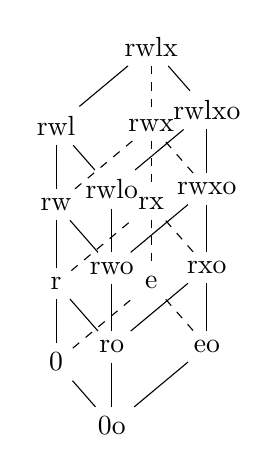
\begin{tikzpicture}[main node/.style={}]
    \node[main node] (rwlx) {$\rwlx$};
    \node[main node] (rwx) [below of=rwlx] {$\rwx$};
    \node[main node] (rx) [below of=rwx] {$\rx$};
    \node[main node] (e) [below of=rx] {$\enter$};


    \node[main node] (rwlxo) [below right of=rwlx,yshift=-0.1cm] {$\rwlxo$};
    \node[main node] (rwxo) [below of=rwlxo] {$\rwxo$};
    \node[main node] (rxo) [below of=rwxo] {$\rxo$};
    \node[main node] (eo) [below of=rxo] {$\entero$};

    \node[main node] (rwl) [below left of=rwlx,xshift=-0.5cm,yshift=-0.3cm] {$\rwl$};
    \node[main node] (rw) [below of=rwl] {$\rw$};
    \node[main node] (r) [below of=rw] {$\readonly$};
    \node[main node] (0) [below of=r] {$\noperm$};

    \node[main node] (rwlo) [below right of=rwl,yshift=-0.1cm] {$\rwlo$};
    \node[main node] (rwo) [below of=rwlo] {$\rwo$};
    \node[main node] (ro) [below of=rwo] {$\ro$};
    \node[main node] (0o) [below of=ro] {$\nopermo$};


    \path[every node/.style={font=\sffamily\small}]
    (rwlxo) edge (rwxo)
    (rwxo) edge (rxo)
    (rxo) edge (eo)

    (rwl) edge (rw)
    (rw) edge (r)
    (r) edge (0)

    (rwlo) edge (rwo)
    (rwo) edge (ro)
    (ro) edge (0o)

    (rwlx) edge[dashed] (rwx)
    (rwx) edge[dashed] (rx)
    (rx) edge[dashed] (e)

    (rwlo) edge (rwlxo)
    (rwo) edge (rwxo)
    (ro) edge (rxo)
    (0o) edge (eo)

    (rwlo) edge (rwl)
    (rwo) edge (rw)
    (ro) edge (r)
    (0o) edge (0)

    (rwl) edge (rwlx)
    (rw) edge[dashed] (rwx)
    (r) edge[dashed] (rx)
    (0) edge[dashed] (e)

    (rwlxo) edge (rwlx)
    (rwxo) edge[dashed] (rwx)
    (rxo) edge[dashed] (rx)
    (eo) edge[dashed] (e);
  \end{tikzpicture}

  \caption{Permission hierarchy}
  \label{fig:perm-hier}
\end{figure}

\subsection{Operational Semantics}
\subsubsection{Notes}
Genrally:
\begin{itemize}
\item Opaque capabilities: Only allow locality and permission to be inspected (i.e., no addresses disclosed).
\end{itemize}

Source language:
\begin{itemize}
\item Variable length instructions that match the length of the compiled instructions
  \begin{itemize}
  \item Opaque capabilities do not hide the length of a program (especially an issue if we ever hope to have error recovery).
  \item This is needed for correctness. See subsection~\ref{subsec:capability-opacity} for an example it helps prevent.
  \end{itemize}
\item Programs have undefined behavior when passing ret/stk pointers.
\end{itemize}

Target language:
\begin{itemize}
\item 
\end{itemize}

\subsubsection{Helpful functions}
\[
  \updPcAddr \defeq \dots
\]

\[
  \updPcPerm \defeq \dots
\]

\[
  \clearms \defeq \dots
\]

\[
  \clearlocreg \defeq \dots
\]

\subsubsection{Source Language}

\begin{align*}
  \ssem{\sjmp{r}} = & 
    \begin{cases}
      \Phi
      \begin{aligned}[t]
        & \update{\sreg.\pcreg}{\opc} \\
        & \update{\smsstk}{\ms_\stk' \uplus \clearms{\ms_\stk}}\\
        & \update{\sastk}{a_\stk'}\\
        & \update{\sstk}{\stk'}
      \end{aligned} & \Phi(r) = \retptr \text{ and }
      \Phi.\sstk = (\opc,\ms_\stk',a_\stk') :: \stk'\\
      & \\
      \updPc{\updPcPerm{\Phi(r)}} & \text{otherwise}
    \end{cases} \\
\end{align*}
\begin{align*}
  \ssem{\scall{r}{\rn}} = & 
    \begin{cases}
      (\mem,\reg',\stk',\ms_\stk') & \Phi = (\mem,\reg,\stk,\ms_\stk) \text{ and }\\
      \\
      \failed & \text{otherwise}
    \end{cases}
\end{align*}

\subsubsection{Target Language}

\subsection{Compiler}
\[
\comp{\cdot} : \src{i}^* \fun \trg{i}^*
\]
\clearpage
\section{Examples}
\subsection{Capability Opacity}
\label{subsec:capability-opacity}
This example was introduced when we envisioned a capability machine with $\spush{}$, $\spop{}$, $\ssload{}{}$, $\scall{}{}$ and $\sreturn$ instructions. The below example is a motivation for having variable length instructions in the source language because if we have enough memory to ``do the same'' in the target language as in the source language, then the below example does not work.

The following pseudo program demonstrates the need of opaque capabilities. If we assume a system with no opaque capabilities, then the following programs break compiler correctness
\begin{lstlisting}[basicstyle=\sourcecolor{}\ttfamily] 
p1 ::= if r1 is length 2 then
         call r1 with the following callback in r5:
           {put $\textit{\texttt{diverging}}$ closure in r2;
            return};
         halt
       else diverge

p2 ::= if r1 is length 2 then
         call r1 with the following callback in r5:
           {put $\textit{\texttt{terminating}}$ closure in r2;
            return};
         halt
       else diverge
\end{lstlisting}
The diverging closure could just contain $\sjmp{\pcreg}$, which diverges. The terminating closure could just be $\sreturn$.

The context with $r1$ as an executable capability pointing to:
\begin{lstlisting}
$\scall{r5}{0}$
$\sjmp{r5}$
\end{lstlisting}
distinguishes the two contexts, but two instructions are not enough to do the same at the target level. We would not have enough instructions to set up a proper return pointer for the compiled return to use.

\clearpage
\section{Back translation}
The back translation is an embedding of source language into .

\section{Notes}
\subsection{Leuven stay conclusions}
\begin{enumerate}
\item Enter capabilities replaces by sealed code/data pairs \label{item:first-point}
  \begin{itemize}
  \item To allow us to forbid dynamic code generation
  \end{itemize}
\item Conditional full-abstraction
  \begin{itemize}
  \item No undefined behaviour by \emph{trusted code} in any context implies full-abstraction. (Blame idea: undefined as undef of current pc, so current pc can be checked for whether it was the trusted code).
  \item Avoids dynamic checks to protect trusted code against itself.
  \item Possible due to point \ref{item:first-point}.
  \end{itemize}
\item replace push/pull/call/ret/sload by symbolic return pointer (pair) and stack pointer.
  \begin{itemize}
  \item Allows backtranslation to be embedding into source language.
    \begin{itemize}
    \item Interpreter for backtranslation is not able to accurately replicate code length.
    \end{itemize}
  \end{itemize}
\item Worlds similar to CSF paper, but invariants on seals as well.
  \begin{itemize}
  \item Invariants says what can be sealed with a certain seals.
  \end{itemize}
\item Linker: resolves symbols
  \begin{itemize}
  \item Export refs (Question: do we allow other things than sealed code/data pairs to be exported?)
  \item Import refs
  \item Fresh seal requirement
  \end{itemize}
\item Components are memory segments and symbols.
\item Variable instruction length in the source to avoid leaking information through code size that cannot be matched after compilation (breaks compiler correctness, se example in subsection~\ref{subsec:capability-opacity}).
  \begin{itemize}
  \item Notice x86 allows instructions of up to infinite length, so this is not weird.
  \end{itemize}
\item Have opaque capabilities.
  \begin{itemize}
  \item Without opaque capabilities, stack consumption could be inferred through stack pointer index etc.
  \end{itemize}
\item Considered PORs for transition systems to: (a->b => a=a and b=b)
  \begin{itemize}
  \item Define one region that governs the stack
  \item Make the regions more general
  \item For now, we have not done this: instead we stick with the transition systems we have and have to regions governing the stack reflecting the CSF work.
  \end{itemize}
\end{enumerate}
\end{document}